\documentclass[acmsmall, nonacm, review]{acmart}

% supress font size warnings
\usepackage{anyfontsize}
\usepackage{fix-cm}

\let\Bbbk\relax % avoid clash

\usepackage{amsmath,amssymb,bm,amsfonts,amsthm,mathtools}
\usepackage[only,llbracket,rrbracket,llparenthesis,rrparenthesis]{stmaryrd}
\usepackage{physics}
\usepackage{mathpartir}
\usepackage{tikz-cd}
\usepackage{qcircuit}
\usepackage{thm-restate}

\usetikzlibrary{positioning, arrows.meta, shapes.multipart, shadows, shapes.geometric, math}

\theoremstyle{plain}
\newtheorem{thm}{Theorem}[section]
\newtheorem{prop}[thm]{Proposition}
\newtheorem{lem}[thm]{Lemma}
\newtheorem{cor}[thm]{Corollary}
\theoremstyle{definition}
\newtheorem{dfn}[thm]{Definition}
\newtheorem{ex}[thm]{Example}
\theoremstyle{remark}
\newtheorem{rem}[thm]{Remark}

\tikzset{
  node distance=1cm and 1.5cm,
  title/.style={
      font=\bfseries\small
    },
  mem/.style={
      rectangle,
      draw,
      thick,
      fill=blue!10,
      minimum height=1cm,
      minimum width=1cm,
      drop shadow
    },
  op/.style={
      ellipse,
      draw,
      thick,
      fill=green!10,
      minimum height=0.6cm,
      minimum width=0.9cm
    },
  arr/.style={
      -Stealth,
      thick
    }
}

\title{A Non-linear Quantum Lambda Calculus}
\author{Rikiya Kashiwagi}
\author{Atsushi Igarashi}
\affiliation{%
  \institution{Kyoto University}
  \department{Graduate School of Informatics}
  \city{Kyoto}
  \country{Japan}
}
\email{kashiwagi@fos.kuis.kyoto-u.ac.jp}
\email{igarashi@kuis.kyoto-u.ac.jp}

\begin{abstract}
  This paper presents a quantum extension of lambda calculus without linearity, reinterpreting contraction and weakening as logical operations on references to quantum states, rather than on the states themselves.
  We formally define the calculus with its operational semantics and conjecture that $\beta$-equal classical terms are contextually equivalent.
  This design enables the seemless integration of classical and quantum programming.
\end{abstract}

%\keywords{quantum programming language, lambda calculus}

\begin{document}
\maketitle

\section{Introduction} \label{sec:intro}
The theoretical foundations of quantum programming languages have largely been built upon linear logic and its variants\cite{VANTONDER2004_LambdaCalculusQuantum,SELINGER2009_QuantumLambdaCalculus,ALTENKIRCH2005_FunctionalQuantumProgramming,SABRY2018_SymmetricPatternMatchingQuantum,ROSS2017_AlgebraicLogicalMethods}, reflecting the \textit{No-Cloning} Theorem\cite{WOOTTERS1982_SingleQuantumCannota} and the \textit{No-Deleting} Theorem\cite{KUMARPATI2000_ImpossibilityDeletingUnknowna} of quantum mechanics.
Within this paradigm, variables representing quantum states are treated as linear resources that can be neither duplicated (contracted) nor discarded (weakened).
While this linearity ensures the physical correctness, it creates a significant gap with the intutions of classical, non-linear programming.

This paper proposes a quantum language designed as a direct extension of the ordinary, non-linear lambda calculus.
Our central design principle is to ensure that ordinary equational reasoning of the (call-by-value) lambda calculus is sound in this extension; specifically, $\beta$-equivalent terms remain operationally indistinguishable in the quantum extension.
This approach ensures any embedded classical program executes with its standard semantics, enabling seamless integration of classical and quantum programs.

A key consequence of enforcing this principle is that the quantum features of the language are cleanly isolated from the classical host.
This quantum-native fragment, consisting of a set of unitary operations, forms a distinct module for expressing quantum control.
This separation provides a natural framework that enables coexistence of the historically separate paradigms of `\textit{Quantum Data, Classical Control}'\cite{SELINGER2004_QuantumProgrammingLanguage} and `\textit{Quantum Data, Quantum Control}'\cite{DÍAZ-CARO2022_QuickOverviewQuantum}.
That means a programmer can compose the main logic in a higher-order classical style, while delegating complex quantum subroutines to specialized, domain-specific modules.
The resulting language provides a familiar framework for classical programmers and, at the same time, introduces a structured and powerful abstraction for high-level quantum-classical programming.


\section{Main idea} \label{sec:main-idea}
To build a quantum language on a non-linear foundation, a reinterpretation of the structural rules---contraction and weakening---is essential.
In conventional linear type systems, contraction is viewed as data duplication and weakening as data deletion.
This interpretation conflicts with the No-Cloning and No-Deleting theorems when the data is a quantum state.

Our approach reinterprets these rules using \textit{reference-based semantics}.
Contraction is not the physical copying of a quantum state, but merely the duplication of a reference to it.
Similarly, weakening is simply the act of dropping a reference.
As these are purely logical operations on references, they do not violate any physical laws.
The physical instantiation of a quantum state occurs only when a unitary operator is applied to one of its duplicated references.
Specifically, if the state is expressed as $\sum_i\alpha_i\ket{i}$, where $\{\ket{i}\}$ is a basis set, and a unitary $U$ is applied, the operation transforms the state into the entangled state $\sum_i\alpha_i\ket{i}(U\ket{i})$.
This is similar to the `\textit{Contraction as sharing}' concept like in \cite{ALTENKIRCH2005_FunctionalQuantumProgramming,ARRIGHI2004_OperationalSemanticsFormal}, but it occurs not at the contraction step, but right before the application of a unitary.

This design has profound consequences for the language's equational theory.
Consider a copy function $\delta \equiv \lambda x.\langle x,x\rangle$ and a projection $\pi_1 \equiv \lambda\langle x,y\rangle.x$.
In our system, the equality $\pi_1\circ\delta=\lambda x. x$ holds.
This is because weakening (via $\pi_1$) is a logical dereference, not a physical act.
In contrast, this identity fails in languages like QML\cite{ALTENKIRCH2005_FunctionalQuantumProgramming} or Qunity\cite{VOICHICK2023_QunityUnifiedLanguage}, where weakening is interpreted as a partial trace.
In those systems, the composition $\pi_1\circ\delta$ induces decoherence, mapping a pure state to a mixed one.

However, this equational property is carefully constrained.
If we define a copy function with inserting an identity unitary, $\delta_I \equiv \lambda x.\langle I\ x,x\rangle$, then $\pi_1\circ\delta_I\ne\lambda x.x$.
The application of the unitary $I$ makes $I\ x$ a distinct physical instance from $x$; for example, the input state $\alpha\ket{0}+\beta\ket{1}$ becomes the entangled state $\alpha\ket{00}+\beta\ket{11}$.
The evaluation procedure for this case is illustrated in Fig.~\ref{fig:grids}.
We can only hope that the equational theory is sound with respect to operational equivalence for the classical fragment without unitaries like $I$.

% This behavior does not violate the soundness mentioned conservativity property of our language.
% Unitary operators like $I$ are separated from the classical fragment.
% The conservativity applies only to the common language, and equational laws are not expected to hold for terms containing unitaries.

\begin{figure}[t]
  \centering
  \begin{minipage}{0.2\textwidth}
    \centering
    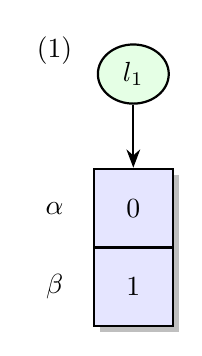
\begin{tikzpicture}
  \draw[step=1cm, color=gray] (0,0) grid (1,2);
  \node (scal) at (-0.5,1.5) {$\alpha$}; \node[mem] (mem1) at (0.5,1.5) {$0$};
  \node at (-0.5,0.5) {$\beta$}; \node[mem] at (0.5,0.5) {$1$};
  \node[op, above=0.8cm of mem1] (op1) {$l_1$};
  \draw[arr] (op1) to (mem1);
  \node[above=1.5cm of scal] {(1)};
\end{tikzpicture}
  \end{minipage}
  \hfill
  \begin{minipage}{0.2\textwidth}
    \centering
    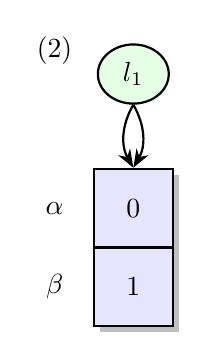
\begin{tikzpicture}
  \draw[step=1cm, color=gray] (0,0) grid (1,2);
  \node (scal) at (-0.5,1.5) {$\alpha$}; \node[mem] (mem2) at (0.5,1.5) {$0$};
  \node at (-0.5,0.5) {$\beta$}; \node[mem] at (0.5,0.5) {$1$};
  \node[op, above=0.8cm of mem2] (op2) {$l_1$};
  \draw[arr, bend left=30] (op2.south) to (mem2.north);
  \draw[arr, bend right=30] (op2.south) to (mem2.north);
  \node[above=1.5cm of scal] {(2)};
\end{tikzpicture}
  \end{minipage}
  \hfill
  \begin{minipage}{0.25\textwidth}
    \centering
    \begin{tikzpicture}
  \draw[step=1cm, color=gray] (0,0) grid (1,2);
  \node at (scal) (-0.5,1.5) {$\alpha$}; \node[mem] (mem1) at (0.5,1.5) {$0$}; \node[mem] (mem2) at (1.5,1.5) {$0$};
  \node at (-0.5,0.5) {$\beta$}; \node[mem] at (0.5,0.5) {$1$}; \node[mem] at (1.5,0.5) {$1$};
  \node[op, above=0.8cm of mem2] (op2) {$l_2$};
  \node[op, above=0.8cm of mem1] (op1) {$l_1$};
  \draw[arr] (op1) to (mem1);
  \draw[arr] (op2) to (mem2);
  \node[above=1.5cm of scal] {(3)};
\end{tikzpicture}
  \end{minipage}
  \hfill
  \begin{minipage}{0.25\textwidth}
    \centering
    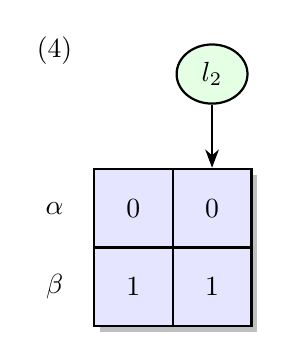
\begin{tikzpicture}
  \draw[step=1cm, color=gray] (0,0) grid (1,2);
  \node (scal) at (-0.5,1.5) {$\alpha$}; \node[mem] (mem1) at (0.5,1.5) {$0$}; \node[mem] (mem2) at (1.5,1.5) {$0$};
  \node at (-0.5,0.5) {$\beta$}; \node[mem] at (0.5,0.5) {$1$}; \node[mem] at (1.5,0.5) {$1$};
  \node[op, above=0.8cm of mem2] (op2) {$l_2$};
  \draw[arr] (op2) to (mem2);
  \node[above=1.5cm of scal] {(4)};
\end{tikzpicture}
  \end{minipage}
  \caption{Illustration of the internal states when $\pi_1\circ\delta_I$ is applied to a qubit. The grids correspond to quantum states. The rows represent composite systems, and the columns represent superposition with the scalers on the left. From left to right: (1) $l_1$ refers to some qubit state. (2) Contraction duplicates a reference, not a state. (3) Applying an identity unitary to one of the duplicated references creates a distinct physical instance . (4) Weakening drops a reference.}
  \Description{Four grid diagrams showing the step-by-step process of applying $\pi_1\circ\delta_I$ to a qubit. Each grid shows quantum states with rows representing composite systems and columns showing superposition states with scalar coefficients. The sequence demonstrates: initial qubit reference, reference duplication through contraction, identity unitary application creating distinct physical instances, and final reference dropping through weakening.}
  \label{fig:grids}
\end{figure}

\section{\texorpdfstring{The $\Lambda(\mathcal{U})$ calculus}{The Lambda(U) calculus}}
\subsection{Syntax}
As outlined in the introduction, our language is designed as a conservative extension of a non-linear lambda calculus denoted by $\Lambda$. $\Lambda$ is a set of terms including lambda terms, the unit and introductions and eliminations of products and sums. The key to our design is the isolation of quantum features from $\Lambda$, which is provided by a set $\mathcal{U}$ of external unitary operations.
\begin{dfn}[The surface language $\Lambda(\mathcal{U})$]
  Given a set of terms $\mathcal{U}$, the language $\Lambda(\mathcal{U})$ is a set of terms defined by the following syntax:
  \begin{equation*}
    \begin{array}{rl}
      M, N, P \Coloneqq & *\mid x\mid\lambda x. M\mid M\ N\mid\langle M, N\rangle\mid\texttt{inj}_0\ M\mid\texttt{inj}_1\ M \mid \\& \texttt{let}\ \langle x, y\rangle=M\ \texttt{in}\ N\mid\texttt{match}\ M\ [x\Rightarrow N\mid y\Rightarrow P]\mid\hat{U}
    \end{array}
  \end{equation*}
  where $\hat{U}\in\mathcal{U}$. Alternatively, $\Lambda(\mathcal{U})$ is defined as $\Lambda\cup\mathcal{U}$.
\end{dfn}

From the perspective of the host language $\Lambda(\cdot)$, $\hat{U}$ is treated as an opaque, first-class value.
The language $\mathcal{U}$ can represent any unitary transformation, ranging from a simple unitary gate to a complex subroutine that could be described by a domain-specific language, such as one based on the 'Quantum Data, Quantum Control' paradigm.
\begin{ex} \label{ex:classical}
  The classical bit can be represented as $i \equiv \texttt{inj}_i\ *$ where $i=0,1$.
  A standard conditional expression $\texttt{if}\ M\ \texttt{then}\ N\ \texttt{else}\ P$ can be written as a syntactic sugar for $\texttt{match}\ M\ [x\Rightarrow N\mid y\Rightarrow P]$, where $x$ and $y$ are fresh variables.
  Using these notations, the logical NOT is $\textit{not} \equiv \lambda x.\texttt{if}\ x\ \texttt{then}\ 1\ \texttt{else}\ 0$, and the logical AND is $\textit{and} \equiv \lambda x.\lambda y.\texttt{if}\ x\ \texttt{then}\ y\ \texttt{else}\ 0$.
\end{ex}
The quantum aspect of the language is captured by the $\hat{U}$ term.
Match expressions need special attention in this context.
It behaves as usual only when the outermost of the scrutinee is evaluated to inl or inr.
When it is evaluated to superposition of inl and inr, it performs a measurement to project one of them before that.
\begin{ex}[Quantum teleportation] \label{ex:teleportation}
  Let $\mathcal{U}$ be $\{H,CNOT,Z,X\}$ as the standard quantum gate set.
  The following program implements the quantum teleportation circuit on the right:
  \begin{center}
    \begin{minipage}{0.40\textwidth}
      \begin{equation*}
        \begin{array}{l}
          \texttt{let}\ \langle a, b\rangle=CNOT\ \langle H\ 0, 0\rangle\ \texttt{in}           \\
          \texttt{let}\ \langle x, y\rangle=CNOT\ \langle q, a\rangle\ \texttt{in}              \\
          \texttt{let}\ b' = \texttt{if}\ y\ \texttt{then}\ X\ b\ \texttt{else}\ b\ \texttt{in} \\
          \texttt{if}\ H\ x\ \texttt{then}\ Z\ b'\ \texttt{else}\ b'
        \end{array}
      \end{equation*}
    \end{minipage}
    \begin{minipage}{0.45\textwidth}
      \centering
      \hspace{1em}
      \Qcircuit @C=0.8em @R=0.8em {
      \lstick{q}       & \qw      & \qw      &           \qw & \ctrl{1} & \ustick{x}\qw &\gate{H}         &            \qw & \meter           & \\
      \lstick{\ket{0}} & \gate{H} & \ctrl{1} & \ustick{a}\qw & \targ    & \ustick{y}\qw &\meter           &                & \cwx             & \\
      \lstick{\ket{0}} & \qw      & \targ{}  & \ustick{b}\qw & \qw      &           \qw &\gate{X}\cwx{-1} & \ustick{b'}\qw & \gate{Z}\cwx{-2} & \qw
      }
    \end{minipage}
  \end{center}
  where $\texttt{let}\ x = M\ \texttt{in}\ N$ is a syntactic sugar for $(\lambda x. N)\ M$.
\end{ex}
It should be noted that the \textit{not} function in Example \ref{ex:classical} does not behave as the $X$ gate (or the quantum NOT gate) when applied to a qubit, because the input is measured in the condition of the if expression, which collapses any superposition.

As a powerful example of this encapsulation of $\mathcal{U}$, a syntax inspired by pattern isomorphism\cite{SABRY2018_SymmetricPatternMatchingQuantum} allows for the direct declaration of unitary operations as follows.
\begin{ex}[Pattern isomorphism for unitaries]
  Let $\mathcal{U}$ be defined using the pattern isomorphism syntax.
  For instance, $X$ gate can be defined as $X \equiv \{0 \leftrightarrow 1\mid 1 \leftrightarrow 0\}$.
\end{ex}
\subsection{Mathematical preliminaries for operational semantics} \label{sec:math-prelim}
Our operational semantics relies on two key mathematical structures: $\ell^2$ \textit{space} to represent quantum states, and \textit{finite distributions} to model probabilistic reduction.

\begin{dfn}[$\ell^2$ space]
  Given a countable set $X$, the $\ell^2$ space is defined as the set:
  \begin{equation*}
    \ell^2(X) := \left\{\psi : X\to\mathbb{C}\ \left|\ \|\psi\| := \sum\nolimits_{x\in X} |\psi(x)|^2 < \infty \right.\right\},
  \end{equation*}
  and inner product $\langle \psi, \phi \rangle = \sum\nolimits_{x\in X} \overline{\psi(x)} \phi(x)$.
  It is known that $(\ell^2(X), \langle\cdot,\cdot\rangle)$ forms a Hilbert space.
\end{dfn}

\begin{dfn}[Finite distributions]
  The set of finite distributions over $X$ is defined as:
  \begin{equation*}
    \mathcal{D}(X) := \left\{\mu : X \to \ [0,1] \left|\ |\mu| := \sum\nolimits_{x\in X} \mu(x) = 1,\ |\mathrm{supp}(\mu)| < \infty\right.\right\}.
  \end{equation*}
\end{dfn}
Any element of $\ell^2(X)$ and $\mathcal{D}(X)$ can be written as linear combinations: $\psi = \sum_{x\in X} \psi(x) \delta_x$ and $\mu = \sum_{x\in X} \mu(x)\delta_x$ respectively, where $\delta_x$ is defined by $\delta_x(y) = 1$ if $y = x$ and $0$ otherwise.

Next, we utilize two linear map constructions for $\ell^2$.
The first is the functorial action of $\ell^2$, which lifts any function $f: X \to Y$ to a linear map $\ell^2(f): \ell^2(X) \to \ell^2(Y)$ defined by $\ell^2(f)(\delta_x) := \delta_{f(x)}$.
The second one extends a function $k: X \to \ell^2(Y)$ to a linear map $k^\sharp: \ell^2(X) \to \ell^2(Y)$ via linear extension: $k^\sharp(\sum_{x \in X} \alpha_x \delta_x) := \sum_{x \in X} \alpha_x k(x)$ only if the resulting sum converges for any input.
\subsection{Operational semantics}
This section defines the operational semantics, describing how the reference-based semantics from Section~\ref{sec:main-idea} is formalized.
The state of a computation is captured by a \textit{configuration}: a pair of a global store and the term being evaluated.
Crucially, the store holds the physical quantum state, while the term operates only on locations ($\mathcal{L}$)---references to that store.
This separation allows contraction and weakening to be treated as logical operations on references, without directly affecting the physical quantum state.
Because a term is rewritten to contain these locations during execution, we must first define a distinct runtime language that extends the surface syntax with them.

\begin{dfn}[The runtime language $\Lambda_\mathcal{L}(\mathcal{U})$]
  Given a set of store locations $\mathcal{L}$, the runtime language is defined as $\Lambda_\mathcal{L}(\mathcal{U}) := \Lambda(\mathcal{U}\cup\mathcal{L})$.
  To simplify notation, $M, N, P$ will also range over runtime terms.
  We will explicitly refer to surface terms when the distinction is significant.
\end{dfn}

Only first-order, or \textit{basis values}, can be placed in the store and exist in a superposition.
Values and basis values are given by the following syntax.
\begin{equation*}
  \begin{array}{lrl}
    \text{Values}       & V, W \Coloneqq             & l \mid *\mid\lambda x. M\mid\langle V, W\rangle\mid\texttt{inj}_0\ V\mid\texttt{inj}_1\ V\mid\hat{U} \\
    \text{Basis values} & \hat{V}, \hat{W} \Coloneqq & *\mid\langle\hat{V}, \hat{W}\rangle\mid\texttt{inj}_0\ \hat{V}\mid\texttt{inj}_1\ \hat{V}
  \end{array}
\end{equation*}
The set of all basis values is denoted by $\mathcal{V}_0$.

A configuration $[\sigma, M]$ represents the state of a computation.
The quantum store $\sigma$ is a vector in a free Hilbert space over value stores (finite maps from locations $\mathcal{L}$ to basis values $\mathcal{V}_0$), while $M$ is the runtime term containing references to $\sigma$.
Each value store in the support of $\sigma$ must have the same domain; we can define $\text{dom}(\sigma)$ without ambiguity.
Write $\mathcal{C}$ for the set of all configurations.

The operational semantics are defined by a call-by-value, small-step reduction relation ($\longrightarrow$).
The key rules in Fig.~\ref{fig:reduction} directly correspond to the four postulates of quantum mechanics\cite{NIELSEN2010_QuantumComputationQuantum}.
\begin{description}
  \item[State preparation (\textsc{Q-Prep})] It prepares a quantum state by taking a classical basis value $\hat{V}$ and placing it into the store at a new location $l$.
  \item[Unitary Evolution (\textsc{Q-Evolve})] Applying a unitary $\hat{U}$ to a reference $l_1$ transforms the entire quantum store $\sigma$ according to the operator's interpretation.
        The location $l_1$ stays in the store, which reflects the 'Contraction as sharing' mechanism as illustrated in Fig.~\ref{fig:grids}.
  \item[Measurement (\textsc{Q-Meas})] The match expression performs a measurement on a referenced state, causing the computation to branch probabilistically and collapsing the quantum store.
  \item[Composite system (\textsc{Q-Destr})] It destructs a pair stored at $l_1$ and creates new, distinct references $l_2$, $l_3$ to its components.
        It copies values at each value store, not meaning that the superpositions themselves are cloned.
\end{description}

This semantics imposes a meta-level constraint on $\hat{U}$.
Specifically, the \textit{interpretation} $\llbracket\hat{U}\rrbracket_\mathcal{U} : \mathcal{V}_0\rightharpoonup \ell^2(\mathcal{V}_0)$ must satisfy the following condition: if $U = \llbracket\hat{U}\rrbracket_\mathcal{U}$, then $(U|_{\mathrm{dom}(U)})^\sharp$ is unitary.
\begin{dfn}[Small-step reduction] \label{def:single-step}
  Given a set of partial functions $\llbracket\hat{U}\rrbracket_\mathcal{U}$ for $\hat{U}\in\mathcal{U}$, the reduction relation $\longrightarrow \subseteq \mathcal{C}\times \mathcal{D}(\mathcal{C})$ is the smallest relation closed under the classical rules (Appendix~\ref{sec:opsem-full}) and the quantum rules (Fig.~\ref{fig:reduction}).
  The relation is then extended to all evaluation contexts $E$ via the standard congruence rule: if $[\sigma,M] \longrightarrow \mu$, then $[\sigma,E[M]] \longrightarrow \sum_{[\sigma',M']\in\mathrm{supp}(\mu)}\mu([\sigma',M'])\delta_{[\sigma',E[M']]}$.
  The definition of evaluation contexts is given in Appendix~\ref{sec:opsem-full}.
\end{dfn}

\begin{figure}[t]
  \centering
  \begin{mathpar}
    \inferrule*[right=Q-Destr]
    {f(\rho) = \rho\cup\{(l_2,\hat{V}),(l_3, \hat{W})\}\text{ where } \rho(l_1) = \langle \hat{V}, \hat{W}\rangle \\ l_2, l_3 \notin \mathrm{dom}(\sigma)}
    {[\sigma, \texttt{let}\ \langle x, y\rangle=l_1\ \texttt{in}\ M] \longrightarrow \delta_{[\ell^2(f)(\sigma), M[l_2/x,l_3/y]]}}
    \and
    \inferrule*[right=Q-Meas]
    {|\alpha_0|^2 + |\alpha_1|^2 = 1 \\ ||\sigma_0|| = ||\sigma_1|| \\ f_0(\rho) = \rho\cup\{(l_2,\hat{V})\}\text{ where } \rho(l_1) = \texttt{inj}_0\ \hat{V} \\ f_1(\rho) = \rho\cup\{(l_3,\hat{W})\}\text{ where } \rho(l_1) = \texttt{inj}_1\ \hat{W} \\ l_2 \notin \mathrm{dom}(\sigma_0) \\ l_3 \notin \mathrm{dom}(\sigma_1)}
    {[\alpha_0\sigma_0 + \alpha_1\sigma_1, \texttt{match}\ l_1\ [y\Rightarrow M\mid z\Rightarrow N]] \\
    \longrightarrow |\alpha_0|^2 \delta_{[\ell^2(f_0)(\sigma_0), M[l_2/y]]} + |\alpha_1|^2\delta_{[\ell^2(f_1)(\sigma_1),N[l_3/z]]}}
    \and
    \inferrule*[right=Q-Prep]
    {f(\rho) = \rho\cup\{(l, \hat{V})\} \\\\ l \notin \mathrm{dom}(\sigma)}
    {[\sigma, \hat{U}\ \hat{V}] \longrightarrow \delta_{[\ell^2(f)(\sigma), \hat{U}\ l]}}
    \and
    \inferrule*[right=Q-Evolve]
    { f(\rho) = \sum\nolimits_{\hat{V}}\llbracket\hat{U}\rrbracket_\mathcal{U}(\rho(l_1))(\hat{V})\delta_{\rho\cup\{(l_2, \hat{V})\}} \\\\ l_2 \notin \mathrm{dom}(\sigma)}
    {[\sigma, \hat{U}\ l_1] \longrightarrow \delta_{[f^\sharp(\sigma),l_2]}}
  \end{mathpar}
  \caption{Quantum reduction rules}
  \Description{Four inference rules defining the quantum reduction steps. The first rule (\textsc{Q-Destr}) describes the decomposition of a pair in the store into two new locations. The second rule (\textsc{Q-Meas}) details the measurement process, branching based on the superposition of states. The third rule (\textsc{Q-Prep}) covers state preparation by placing a basis value into the store. The fourth rule (\textsc{Q-Evolve}) explains the application of a unitary operator to a location, transforming the quantum state accordingly.}
  \label{fig:reduction}
\end{figure}

A key property to the physical realizability of the semantics is norm preservation, which guarantees that the norm of the quantum state does not change during reduction.
\begin{restatable}[Norm preservation]{thm}{NormpresTheorem} \label{thm:norm-pres}
  If $[\sigma,M] \longrightarrow \mu$, then for all $[\sigma',M']\in\mathrm{supp}(\mu)$, $||\sigma'|| = ||\sigma||$.
\end{restatable}

Since a single reduction step can yield a distribution of configurations, the \textit{multi-step reduction} ($\longrightarrow^*$) is not a simple reflexive and transitive closure. Instead, it is defined inductively to compose these probabilistic outcomes, akin to a monadic bind.
\begin{dfn}[Multi-step reduction]
  The multi-step reduction relation $\longrightarrow^*\subseteq \mathcal{C}\times \mathcal{D}(\mathcal{C})$ is the smallest relation satisfying:
  \begin{itemize}
    \item $[\sigma,M] \longrightarrow^*\delta_{[\sigma,M]}$ for all $[\sigma,M]\in\mathcal{C}$.
    \item If $[\sigma,M] \longrightarrow \mu$ and for all $[\sigma',M']\in\mathrm{supp}(\mu)$, $[\sigma',M'] \longrightarrow^*\nu_{\sigma',M'}$, then $[\sigma,M] \longrightarrow\sum_{[\sigma',M']\in\mathrm{supp}(\mu)} \mu([\sigma',M'])\nu_{\sigma',M'}$.
          % Each reduction step has finite probablistic branches; thus the summation is well-defined.
  \end{itemize}
\end{dfn}

\begin{dfn}[Termination]
  A surface term $M$ is said to \emph{terminate}, denoted $M\Downarrow$, if there exists $\mu : \mathcal{V} \to [0,1]$ such that $[\delta_\emptyset, M] \longrightarrow\mu$, and for every $[\sigma, M'] \in \mathrm{supp}(\mu)$, $M'$ is a closed value.
\end{dfn}

\subsection{Preservation of Classical Reasoning}
As mentioned in Section \ref{sec:intro}, the central design principle of our language is that the quantum extension preserves the behavior of the classical fragment.
This guarantee is essential for programmers and compilers, as it ensures that classical reasoning and standard optimizations remain valid.
To formalize this, we first define contextual equivalence, which states that two terms are equivalent if their observable behaviors are identical in any context.
A context $C[\cdot]$ is defined as a closed term with a single hole $[\cdot]$ in it.
\begin{dfn}[Contextual equivalence] \label{def:contextual-equiv}
  For $M, N \in \Lambda$, $M\approx N \Leftrightarrow_\mathrm{def} \forall C[\cdot]\in\Lambda(\mathcal{U}).\ C[M] \Downarrow \Leftrightarrow C[N] \Downarrow$.
\end{dfn}

Our main result shows that any classical $\beta$-equivalence is preserved in the full quantum language. Here, $\longleftrightarrow^*_\Lambda$ denotes the congruence closure of the classical reduction relation defined in Appendix~\ref{sec:opsem-full}.
\begin{restatable}[Preservation of $\beta$-equivalence]{thm}{ConservTheorem} \label{thm:conservativity}
  For all $M, N \in \Lambda$, if $M \longleftrightarrow^*_\Lambda N$ then $M \approx N$.
\end{restatable}

%This property cannot be proved for general operational equivalence other than $\beta$-equivalence since our language yields side-effects through measurement.
%Actually, $\eta$-equivalence of \texttt{match} does not hold in general.
%Consider the term $\texttt{match}\ x\ [y\Rightarrow \texttt{inj}_0\ y\mid z\Rightarrow \texttt{inj}_1\ z]$.
%In classical reduction, it is $\eta$-equivalent to $x$.
%However, $x$ can store a quantum state, and thus measuring it results in a probabilistic outcome.
\section{Discussion}

\begin{itemize}
\item Prove the conjecture (cite Dal Lago's work); discuss soundness of $\eta_V$-equivalence.
\item Discuss that the present semantics consumes too many qubits.
  This is OK as the proposed calculus is a semantic basis.  For
  implementation, we need some kind of garbage collection (?).
\end{itemize}

This paper established that classical $\beta$-equivalence is preserved by contextual equivalence ($\leftrightarrow_\beta \Rightarrow \approx$), which justifies applying classical optimizations to the classical fragment.
However, the converse, and thus a full conservative extension result for observational equivalence, fails.
This is a necessary design choice, as the observational effect of measurement breaks $\eta$-equivalence for constructs like match, i.e., $\texttt{match}\ x\ [y\Rightarrow \texttt{inj}_0\ y\mid z\Rightarrow \texttt{inj}_1\ z] \not\approx x$.
The true conservative extension property should relate the equational theories of the two calculi.
Formulating this remains a significant open problem, as our probabilistic reduction relation ($[\sigma, M] \longrightarrow \mu$) requires a novel definition of an equivalence closure that can operate on distributions, a topic we leave for future investigation.


%We aim to develop both practical compilation techniques and theoretical extensions.
%An intermediate language will be designed to explicitly describe interactions between classical and quantum systems through lower-level quantum operations.
%Although the simply typed system is presented in Appendix~\ref{sec:type-system}, it can be extended with polymorphism and recursive types.
%We are also working on a denotational semantics to formalize the language's mathematical interpretations.


\bibliographystyle{ACM-Reference-Format}
\bibliography{references}

\appendix
\section{Operational semantics}
\subsection{Full definitions of operational semantics} \label{sec:opsem-full}
The remaining part of the single-step reduction relation (Definition~\ref{def:single-step}) is the classical $\beta$-reduction rules, given in Fig.~\ref{fig:reduction-beta}.
These rules are standard for call-by-value lambda calculus, and do not interact with the quantum store.
$\dot{V}$ and $\dot{W}$ in the rules denote values with locations.
\begin{figure}[ht]
  \begin{mathpar}
    \inferrule*[right=$\beta$-Lam]
    {}
    {[\sigma,(\lambda x. \dot{M})\ \dot{V}] \longrightarrow [\sigma,\dot{M}[\dot{V}/x]]}
    \and
    \inferrule*[right=$\beta$-Pair]
    {}
    {[\sigma,\texttt{let}\ \langle x,y\rangle=\langle \dot{V},\dot{W}\rangle\ \texttt{in}\ \dot{M}] \longrightarrow [\sigma,\dot{M}[\dot{V}/x,\dot{W}/y]]}
    \and
    \inferrule*[right=$\beta$-Inj$_0$]
    {}
    {[\sigma,\texttt{match}\ \texttt{inj}_0\ \dot{V}\ [x\Rightarrow \dot{M}\mid y\Rightarrow \dot{N}]] \longrightarrow [\sigma,\dot{M}[\dot{V}/x]]}
    \and
    \inferrule*[right=$\beta$-Inj$_1$]
    {}
    {[\sigma,\texttt{match}\ \texttt{inj}_1\ \dot{V}\ [x\Rightarrow \dot{M}\mid y\Rightarrow \dot{N}]] \longrightarrow [\sigma,\dot{N}[\dot{V}/y]]}
  \end{mathpar}
  \caption{Classical reduction rules}
  \label{fig:reduction-beta}
  \Description{A set of inference rules defining basic beta reduction in the operational semantics. The rules include beta reduction for lambda abstraction, product types, and sum types with two cases for injections. Each rule shows how a term in a specific form reduces to another term by substituting values for variables.}
\end{figure}

The relation $\longrightarrow$ is defined by the rules in Fig.~\ref{fig:reduction} and Fig.~\ref{fig:reduction-beta}, together with the congruence rule induced by the evaluation context.
The evaluation contexts are defined as:
\begin{equation*}
  \begin{array}{rl}
    E \Coloneqq & [\cdot]\mid E\ M\mid V\ E\mid\langle E, M\rangle\mid\langle V,E\rangle\mid\texttt{inj}_0\ E\mid\texttt{inj}_1\ E\mid \\
                & \texttt{let}\ \langle x,y\rangle=E\ \texttt{in}\ M\mid\texttt{match}\ E\ [x\Rightarrow M\mid y\Rightarrow N ]
  \end{array}
\end{equation*}

\subsection{Proof of norm preservation}
\begin{lem}[Linearity of norm] \label{lem:norm-linear}
  $\|\sum_i \alpha_i \psi_i\| = \sqrt{\sum_i |\alpha_i|^2 \|\psi_i\|^2}$ if $\langle \psi_i, \psi_j\rangle = 0$ for all $i\ne j$.
\end{lem}

\begin{lem} \label{lem:functor-norm}
  For all injection $f:X\to Y$ and $\psi\in \ell^2(X)$, $\|\ell^2(f)(\psi)\| = \|\psi\|$.
\end{lem}
\begin{proof}
  Let $g$ be a left inverse of $f$, then
  \begin{equation}
    \|\ell^2(f)(\psi)\| = \left\|\sum_{x\in X} \psi(x) \delta_{f(x)}\right\| = \sum_{y\in f(X)} |\psi(g(y))|^2 = \sum_{x\in X} |\psi(x)|^2 = \|\psi\|.
  \end{equation}
\end{proof}

\begin{lem} \label{lem:isometry-norm}
  For all isometry $f:\ell^2(X)\to\ell^2(Y)$ and $\psi\in \ell^2(X)$, $\|f(\psi)\| = \|\psi\|$.
\end{lem}
\begin{proof}
  For all $x, x'\in X$, $\langle f(\delta_x), f(\delta_{x'})\rangle = \langle \delta_x, \delta_{x'}\rangle = 0$ holds because $f$ is an isometry.
  Then, by Lemma~\ref{lem:norm-linear},
  \begin{equation*}
    \|f(\psi)\| = \left\|\sum_{x\in X} \psi(x)f(\psi)\right\| = \sqrt{\sum_{x\in X} |\psi(x)|^2\|f(\delta_x)\|^2}.
  \end{equation*}
  As $\|f(\delta_x)\| = \sqrt{\langle f(\delta_x), f(\delta_x)\rangle} = \|\delta_x\| = 1$, we have $\|f(\psi)\| = \sqrt{\sum_{x\in X} |\psi(x)|^2} = \|\psi\|$.
\end{proof}

\NormpresTheorem*
\begin{proof}
  By induction on the derivation of $[\sigma,M] \longrightarrow \mu$.
  We only show the cases for the quantum rules; the other cases are immediate.
  \begin{itemize}
    \item Case \textsc{Q-Destr}: Since the function $f$ adds new entries $l_2$ and $l_3$ to $\rho$, it is injective; hence by Lemma~\ref{lem:functor-norm}, $\|\ell^2(f)(\sigma)\| = \|\sigma\|$.
    \item Case \textsc{Q-Prep}: The same reasoning as in Case \textsc{Q-Destr}.
    \item Case \textsc{Q-Meas}: Similar argument to the Case \textsc{Q-Destr}, $f_0$ and $f_1$ are injective.
          For each basis $\rho_i$ in $\sigma_i$ ($i=0,1$), $\rho_0 \ne \rho_1$ holds because they differ at least on the values stored in $l_1$; thus, $\langle \sigma_0, \sigma_1\rangle = 0$.
          \begin{align*}
            \|\alpha_0\sigma_0 +\alpha_1\sigma_1\|
             & = \sqrt{|\alpha_0|^2 \|\sigma_0\|^2+|\alpha_1|^2 \|\sigma_1\|^2} \tag{by Lemma~\ref{lem:norm-linear}} \\
             & = \sqrt{(|\alpha_0|^2 + |\alpha_1|^2) \|\sigma_0\|^2} \tag{$\|\sigma_0\| = \|\sigma_1\|$}             \\
             & = \|\sigma_0\| \tag{$|\alpha_0|^2 + |\alpha_1|^2 = 1$}                                                \\
             & = \|\ell^2(f_0)(\sigma_0)\| \tag{by Lemma \ref{lem:functor-norm}}
          \end{align*}
          Similarly, $\|\alpha_0\sigma_0 +\alpha_1\sigma_1\| = \|\ell^2(f_1)(\sigma_1)\|$.
    \item Case \textsc{Q-Evolve}: As $(\llbracket\hat{U}\rrbracket_\mathcal{U})^\sharp$ is a unitary, $\|\llbracket\hat{U}\rrbracket_\mathcal{U}(\rho(l_1))\|^2 = 1$; hence, $\|f(\rho)\| = 1$ for any basis $\rho$ in $\sigma$.
          % Proof of isometry
          For all basis $\rho, \rho'$ in $\sigma$,
          \begin{equation*}
            \langle f(\rho), f(\rho')\rangle = \sum_{\hat{V}}\overline{\llbracket\hat{U}\rrbracket_\mathcal{U}(\rho(l_1))(\hat{V})}\llbracket\hat{U}\rrbracket_\mathcal{U}(\rho'(l_1))(\hat{V}) = \langle \delta_\rho, \delta_{\rho'}\rangle.
          \end{equation*}
          As $f^\sharp(\delta_\rho) = f(\rho)$ by definition, $\langle f^\sharp(\delta_\rho), f^\sharp(\delta_{\rho'})\rangle = \langle \delta_\rho, \delta_{\rho'}\rangle$ holds, which means $f^\sharp$ is an isometry.
          Thus, by Lemma~\ref{lem:isometry-norm}, $\|f(\sigma)\| = \|\sigma\|$.
  \end{itemize}
\end{proof}
\section{Proof of Theorem \ref{thm:conservativity}} \label{sec:conserv-proof}
Church-Rosser property for the classical reduction directly follows from the determinism of $\longrightarrow_\Lambda$.
\begin{lem}[Church-Rosser for classical reduction] \label{lem:classical-CR}
  For any $M, N \in \Lambda$, if $M \longleftrightarrow^*_\Lambda N$ holds, then there exists $P \in \Lambda$ such that $M \longrightarrow^*_\Lambda P$ and $N \longrightarrow^*_\Lambda P$.
\end{lem}

\ConservTheorem*
\begin{proof}[Proof]
  By applying Lemma \ref{lem:classical-CR}, there exists $P \in \Lambda$ such that $M \longrightarrow^*_\Lambda P$ and $N \longrightarrow^*_\Lambda P$.
  Then, by congruence condition of $\longrightarrow^*$, $[\sigma, E[M]] \longrightarrow^* \delta_{[\sigma, E[P]]}$ and $[\sigma, E[N]] \longrightarrow^* \delta_{[\sigma, E[P]]}$ hold for any $\sigma$.
  Therefore, we can state that $E[M]\Downarrow$ iff $E[N]\Downarrow$.
\end{proof}
\section{Type system} \label{sec:type-system}
We present the simple type system of $\Lambda(\mathcal{U})$ calculus.
Syntax of types and typing context is given as follows.
\begin{equation*}
  \begin{array}{lrl}
    \text{Types}          & A, B, C \Coloneqq          & \top\mid A\otimes B\mid A\oplus B\mid A\rightarrow B    \\
    \text{Basis types}    & \hat{A}, \hat{B} \Coloneqq & \top\mid\hat{A}\otimes \hat{B}\mid\hat{A}\oplus \hat{B} \\
    \text{Typing context} & \Gamma \Coloneqq           & \epsilon \mid \Gamma,x:A                                \\
  \end{array}
\end{equation*}
The types include the unit type $\top$, product types $A \otimes B$, sum types $A \oplus B$, and function types $A \rightarrow B$.
$\otimes$ and $\oplus$ indicate that they are tensor product and direct sum of Hilbert spaces when interpreted as superpositions.
Crucially, there is no distinction between classical and quantum types in this system.
For instance, the type of both classical bit and qubit are represented as the same $\top \oplus \top$.

Typing judgements are defined on the runtime terms, which means they include typing rules for store locations.
In order to map locations to their types, we introduce the notion of store typing.
\begin{dfn}[Store typing]
  A store typing $\Sigma$ is a finite mapping from locations to basis types.
  A store $\sigma$ is well-typed under $\Sigma$, denoted $\vdash \sigma : \Sigma$, if for every $l\in\text{dom}(\Sigma)$, $\vdash \sigma(l) : \Sigma(l)$ holds.
\end{dfn}

Similar to the definition of the reduction relation, we assume a typing judgement for $\hat{U}\in\mathcal{U}$ in the form of $\vdash_\mathcal{U} \hat{U} : \hat{A} \rightarrow \hat{B}$.
\begin{dfn}[Typing judgments]
  Given a set of external typing judgements $\vdash_\mathcal{U} \hat{U} : \hat{A} \rightarrow \hat{B}$ for $\hat{U}\in\mathcal{U}$,
  A typing judgment is of the form $\Sigma \mid \Gamma \vdash \dot{M} : A$.
  The typing rules are given in Fig.~\ref{fig:typing}.
\end{dfn}

\begin{figure}[t]
  \begin{mathpar}
    \inferrule*[right=Loc]
    { l\in\text{dom}(\Sigma) }
    { \Sigma\mid\Gamma \vdash l : \Sigma(l) }
    \and
    \inferrule*[right=$\top$-I]
    {  }
    { \Sigma\mid\Gamma \vdash * : \top }
    \and
    \inferrule*[right=$\pi_1$]
    { }
    { \Sigma\mid\Gamma,x : A \vdash x : A }
    \and
    \inferrule*[right=$\pi_2$]
    { \Sigma\mid\Gamma \vdash x : A }
    { \Sigma\mid\Gamma,y : B \vdash x : A }
    \and
    \inferrule*[right=$\rightarrow$-I]
    { \Sigma\mid\Gamma, x : A \vdash \dot{M} : B }
    { \Sigma\mid\Gamma \vdash \lambda x.\dot{M} : A\rightarrow B }
    \and
    \inferrule*[right=$\rightarrow$-E]
    { \Sigma\mid\Gamma \vdash \dot{M} : A \rightarrow B \\
      \Sigma\mid\Gamma \vdash \dot{N} : A }
    { \Sigma\mid\Gamma \vdash \dot{M}\ \dot{N} : B }
    \and
    \inferrule*[right=$\otimes$-I]
    { \Sigma\mid\Gamma \vdash \dot{M} : A \\
      \Sigma\mid\Gamma \vdash \dot{N} : B }
    { \Sigma\mid\Gamma \vdash \langle \dot{M},\dot{N}\rangle : A\otimes B }
    \and
    \inferrule*[right=$\oplus_0$-I]
    { \Sigma\mid\Gamma \vdash \dot{M} : A }
    { \Sigma\mid\Gamma \vdash \texttt{inj}_0\ \dot{M} : A\oplus B }
    \and
    \inferrule*[right=$\oplus_1$-I]
    { \Sigma\mid\Gamma \vdash \dot{M} : B }
    { \Sigma\mid\Gamma \vdash \texttt{inj}_1\ \dot{M} : A\oplus B }
    \and
    \inferrule*[right=Op]
    { \vdash_\mathcal{U} \hat{U} : \hat{A} \rightarrow \hat{B} }
    { \Sigma\mid\Gamma \vdash \hat{U} : \hat{A} \rightarrow \hat{B} }
    \and
    \inferrule*[right=$\otimes$-E]
    { \Sigma\mid\Gamma \vdash \dot{M} : A\otimes B \\
      \Sigma\mid\Gamma,x:A,y:B \vdash \dot{N} : C }
    { \Sigma\mid\Gamma \vdash \texttt{let}\ \langle x,y\rangle=\dot{M}\ \texttt{in}\ \dot{N} : C }
    \and
    \inferrule*[right=$\oplus$-E]
    { \Sigma\mid\Gamma \vdash \dot{M} : A \oplus B \\
    \Sigma\mid\Gamma, x : A \vdash \dot{N} : C \\
    \Sigma\mid\Gamma, y : B \vdash \dot{P} : C }
    { \Sigma\mid\Gamma \vdash \texttt{match}\ \dot{M}\ [x\Rightarrow \dot{N}\mid y\Rightarrow \dot{P}] : C }
  \end{mathpar}
  \caption{Typing rules}
  \label{fig:typing}
  \Description{A set of inference rules defining the typing rules for the Lambda(U) calculus. The rules cover typing for locations, unit type, variable projection, lambda abstraction and application, tensor product introduction and elimination, sum type introduction and elimination, and operations from the set of unitaries. Each rule specifies how a term can be assigned a type based on its structure and the types of its components.}
\end{figure}

% safety properties
We can show the standard type safety properties, i.e., subject reduction and progress.
\begin{thm}[Subject reduction]
  If $\Sigma\mid\Gamma \vdash \dot{M} : A$, $[\sigma,\dot{M}] \to [\sigma',\dot{M}']$ and $\vdash \sigma : \Sigma$,
  then there exists $\Sigma'$ such that $\Sigma' \mid \Gamma \vdash M^{*'} : A$ and $\vdash \sigma' : \Sigma'$.
\end{thm}

\begin{thm}[Progress]
  If $\Sigma \mid \Gamma \vdash \dot{M} : A$,
  then either $\dot{M}$ is a value or there exists $\mu$ such that $[\sigma,\dot{M}] \to \mu$.

\end{thm}

%%% Local Variables:
%%% mode: LaTeX
%%% TeX-master: "main"
%%% End:


\end{document}
